%%%%%%%%%%%%%%%%%%%%%%%%%%%%%%%%%%%%%%%%%%%%%%%%%%%%%%%%%%%%%%%%%%%%%%%%%%
\chapter{Optimalizace velikosti bajtkódu}\label{Optimization}

V~této kapitole analyzuji obsah vybraného vzorku \texttt{class} souborů a na základě zjištěných poznatků navrhuji metody pro optimalizaci jejich velikosti. 

%%%%%%%%%%%%%%%%%%%%%%%%%%%%%%%%%%%%%%%%%%%%%%%%%%%%%%%%%%%%%%%%%%%%%%%%%%
\section{Analýza bajtkódu}\label{Optimization:Analysis}

Pomocí nástroje \texttt{jbyca} jsem získala data reprezentující vybraný vzorek testovacích souborů a tato data následně zpracovala a vyhodnotila. Zkoumala jsem velikosti položek v~\texttt{class} souborech, užití lokálních proměnných a parametrů metod a typické sekvence instrukcí. Testovací vzorek jsem vytvořila z~\texttt{jar} souborů stažených z~\texttt{http://mvnrepository.com}. Soubory jsem vybírala náhodně s~ohledem na jejich velikost a četnost stahování. Zvolený vzorek se skládal z~95 souborů o~celkové velikosti 102,4 MB a obsahoval 59 230 \texttt{class} souborů.

\subsection{Velikost položek v~souboru}

Typický \texttt{class} soubor z~velkého vzorku obsahuje v~průměru 117 konstant v~tabulce konstant, 2 členské proměnné, 8 metod, 163 instrukcí a 29 atributů. Ze zkoumání celkové velikosti těchto položek vyplynulo, že konstanty tvoří 64\% z~celkové velikosti všech souborů, struktury pro členské proměnné 1\%, struktury pro metody 2\% a samotné instrukce 10\%.
Nejvýznamnějšími atributy jsou pak \texttt{Code} s~velikostí 30\%, informativní atributy s~velikostí 14\% a \texttt{StackMapTable} s~velikostí 2\%. Velikosti atributů vychází z~délek atributů a velikosti konstant z~tabulky konstant v~nich nejsou zahrnuty.

Při bližším pohledu na velikosti konstant se ukázalo, že 89\% z~celkové velikosti konstant je tvořen pouze konstantami typu \textit{constant\_utf8}. Tedy konstantami popisujícími řetězce v~souboru. Z~těchto řetězců pak 61\% obsahuje názvy tříd, metod a členských proměnných a popisy jejich typů. Konstanty popisující číselné a řetězcové hodnoty tvoří 1\% z~celkové velikosti konstant a zbývající konstanty pro popisy tříd, metod a proměnných tvoří 10\%.

Zkoumání instrukcí z~hlediska jejich velikosti ukázalo, že prvních pět nejobjemnějších instrukcí tvoří 40\% z~celkové velikosti instrukcí. Jsou to instrukce pro volání metod, načtení hodnoty z~členské proměnné a načtení reference na objekt z~lokální proměnné s~indexem 0. Na této pozici se často vyskytuje reference na aktuální objekt. Z~instrukcí s~proměnnou délkou má instrukce \texttt{tableswitch} v~průměru velikost 107 B a instrukce \texttt{lookupswitch} velikost 43 B.

\subsection{Užití lokálních proměnných a parametrů metody}

Data popisující užití parametrů a lokálních proměnných jsou znázorněna v~grafech \ref{fig:params} a \ref{fig:vars}. Z~dat vyplývá, že z~lokálních proměnných obsahujících argumenty metody se tyto hodnoty načtou průměrně jedenkrát a dále se s~nimi nepracuje. S~nižším indexem proměnné počet načítání roste až k~hodnotě 2,5 pro index 0. V~tomto indexu se u~nestatických metod předává reference na aktuální objekt (\texttt{this}). S~lokálními proměnnými, které neslouží k~předávání parametrů, se průměrně provádí 4,2 operací načítání, 1,8 operací vkládání a 0,3 operací inkrementace.

\begin{figure}[h!]
\centering
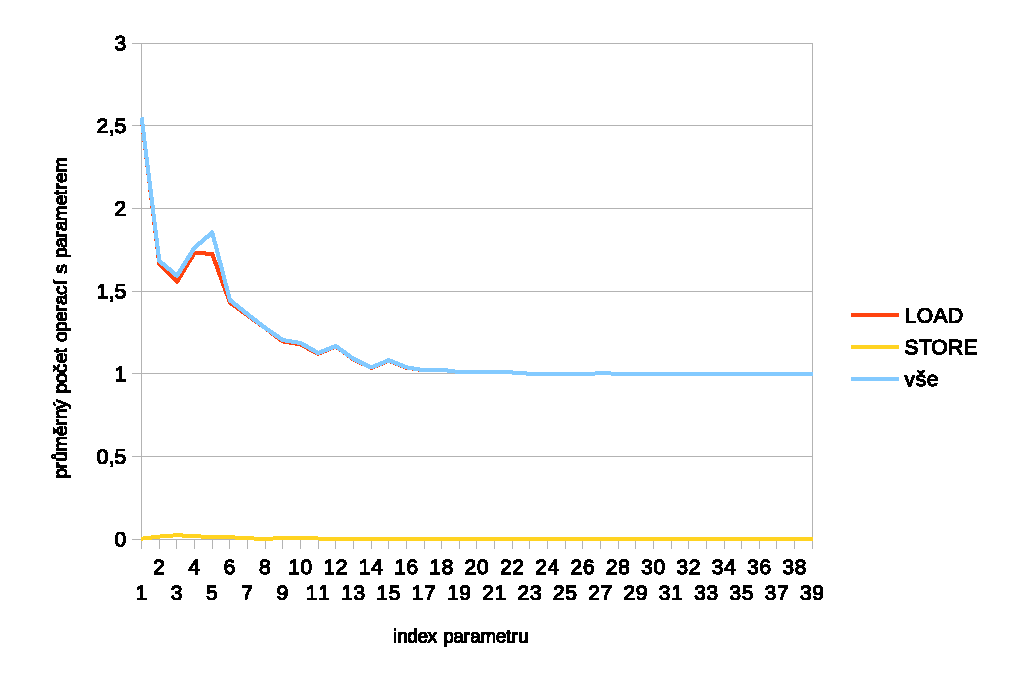
\includegraphics[scale=0.9]{fig/params}
\caption{Průměrné počty operací s~parametry metod.}\label{fig:params}
\end{figure}

\begin{figure}[h!]
\centering
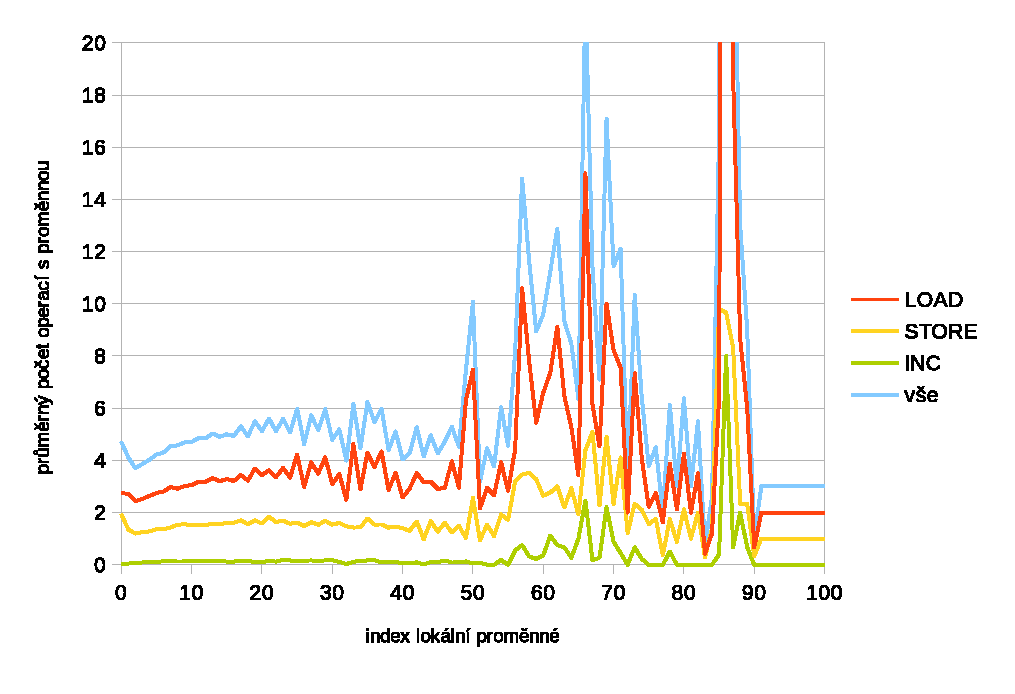
\includegraphics[scale=0.9]{fig/locals} 
\caption{Průměrné počty operací s~lokálními proměnnými.}\label{fig:vars}
\end{figure}

% TODO vzory
\subsection{Typické sekvence instrukcí}

Procentuální ohodnocení sekvence instrukcí se vztahuje k~počtu instrukcí a udává, kolik procent z~celkového počtu instrukcí tvoří daná sekvence. 

\subsubsection{Typické operace}

Z~dat pro sekvence instrukcí délky jedna vyplývá, že 15,69\% instrukcí tvoří instrukce pro volání metod objektu. 
Dalšími významnými instrukcemi jsou instrukce pro čtení hodnot z~lokálních proměnných: čtení z~parametru metody 10,34\%, čtení z~lokální proměnné 5,60\% a čtení reference na aktuální objekt 9,00\%. Na druhou stranu instrukcí pro ukládání hodnot do proměnných je výrazně méně: uložení do lokální proměnné 2,82\%, uložení do parametru metody 1,39\% a v~49 případech byla hodnota uložena do reference na \texttt{this}. To poukazuje opakované načítání neměnících se hodnot. Obdobně instrukce pro načtení a uložení hodnoty z~členské proměnné tvoří 4,50\% a 1,69\%. Pro statické členské proměnné je to 1,15\% a 0,29\%. 

Nejčastější instrukcí skoku je nepodmíněný skok 1,76\%. Následují skoky s~podmínkou rovnosti s~nulou 1,21\%, rovnosti s~\texttt{null} 0,52\% a nerovnosti s~nulou 0,49\%. Z~hlediska práce se zásobníkem jsou zajímavé instrukce pro duplikaci a odebrání vrcholu, které tvoří 3,51\% a 0,88\%. Pro práci s~polem pak instrukce pro uložení hodnoty 1,68\%, načtení hodnoty 0,62\% a zjištění délky pole 0,27\%. Ukládání hodnot do pole je tedy častější operací než čtení hodnot z~pole. U~proměnných to bylo naopak. Instrukce pro návrat z~metody tvoří 4,75\% instrukcí a instrukce pro vytvoření nového objektu 1,96\%.

Za zmínku dále stojí instrukce \texttt{swap} s~2 315 výskyty, \texttt{nop} s~364 výskyty a instrukce \texttt{lookupswitch} a \texttt{tableswitch}. Ve 21 případech instrukce \texttt{lookupswitch} obsahovala jen adresu výchozího bloku instrukcí, v~552 případech obsahovala jednu dvojici hodnota-adresa a v~998 případech dvě dvojice, což je nejčastější podoba této instrukce. V~instrukci \texttt{tableswitch} se nejčastěji pracuje s~rozsahem hodnot o~délce tři a to ve 442 případech. Ve 150 případech byla délka rozsahu 1.

\subsubsection{Typické parametry}

Nejčastěji načítanými typy konstant jsou \texttt{int} 5,87\%, řetězec 2,44\%, reference na \texttt{null} 0,61\%, \texttt{double} 0,24\% a \texttt{long} 0,24\%.
Ze zkoumání konkrétních parametrů instrukcí pak vyplývá, že typickými konstantními hodnotami typu \texttt{int} jsou 0, 1, 2, 3, 4, -1, 8, 5, 6, 10, 7, 16 a 255. Pro typ \texttt{long} jsou to hodnoty 0, 1, -1, pro typ \texttt{double} 0, 1 a pro typ \texttt{float} 0, 1, 0,75 a 2. Typickou řetězcovou konstantou je prázdný řetězec. 

Nejčastější volanou metodou je metoda \texttt{append} třídy \texttt{java.lang.StringBuilder} pro připojení řetězce. Následují metody \texttt{toString} a \texttt{<init>} téže třídy. Metoda \texttt{<init>} třídy \texttt{java.lang.Object} je až čtvrtá v~pořadí. Dále se nejčastěji pracuje s~metodami a objekty tříd \texttt{java.lang.StringBuffer}, \texttt{java.util.Iterator} a \texttt{java.lang.String}.

Typické je jednorozměrné pole typu \texttt{java.lang.Object}, \texttt{java.lang.String} nebo \texttt{byte}. Největší nalezená dimenze vícerozměrného pole byla 3. Typickými konstantními počty prvků v~poli jsou hodnoty 0, 1, 2, 3. Nejčastěji se pracuje s~nultým prvkem pole.

\subsubsection{Typická těla metod}

Celkem 39 317 ze 504 741 zkoumaných metod bylo abstraktních nebo byly metodami rozhraní. Dalších 5 687 metod obsahovalo pouze instrukci pro návrat z~metody. Metody nejčastěji slouží k~získání hodnoty z~členské proměnné aktuálního objektu, volání metody aktuálního objektu a získání konstantní hodnoty. Ze zkoumání metod s~konkrétními operačními kódy a parametry vyplývá, že 6 431 metod jsou implicitními konstruktory. Dalších 2 880 metod vrací hodnotu 0 typu \texttt{int} a 2 261 metod vrací hodnotu 1 typu \texttt{int}. Ve 1 474 případech pak metoda pouze vyvolá výjimku \texttt{UnsupportedOperationException}.


\subsubsection{Zajímavé sekvence instrukcí}

Z~výstupů analýzy typických sekvencí instrukcí jsem vybrala některé zajímavé sekvence, ze kterých lze vycházet při návrhu metod pro optimalizaci velikosti bajtkódu. 
Například vybrané sekvence pro práci se zásobníkem z~tabulky \ref{tab:examples:stack} poukazují na instrukce, které lze snadno odstranit, a na nedostatečné používání specializovaných instrukcí pro manipulaci se zásobníkem.

\begin{table}%[ht]
\begin{texamples}

57 899
& \code{astore $var$; \\ aload $var$;} 
& \desc{Hodnota z~vrcholu zásobníku se uloží do lokální proměnné a následně se načte zpět na zásobník.} \\


26 694
& \code{aload $this$; \\ aload $this$;} 
& \desc{Za zásobník se dvakrát vkládá reference na aktuální objekt.} \\

7 637
& \code{pop; \\ return;} 
& \desc{Manipuluje se se zásobníkem, ačkoliv na jeho stavu nezáleží.} \\

4 023
& \code{aload $var$; \\ pop;} 
& \desc{Na zásobník se vloží hodnota a hned se odebere.} \\

909
& \code{aload $var$; \\ aload $this$; \\ swap;} 
& \desc{Instrukci \texttt{swap} lze aplikovat prohozením instrukcí.} \\

527
& \code{bipush $i$; \\ bipush $i$;} 
& \desc{Za zásobník se dvakrát vkládá ta stejná hodnota.} \\

222
& \code{aload $par$; \\ new $type$; \\ dup\_x1; \\ swap;} 
& \desc{Sekvence typická pro balíček \texttt{groovy}.} \\

\end{texamples}

\caption{Sekvence instrukcí manipulující se zásobníkem.}
\label{tab:examples:stack}
\end{table}


Z~tabulky \ref{tab:examples:numbers} vyplývá, že po vkládání číselných konstant se nemusí používat nejkratší varianty instrukcí. Dále je možné zjednodušit některé algebraické operace na základě jejich vlastností, ale žádné operace nad konstantními hodnotami v~bajtkódu nalezeny nebyly. Stejně tak nebyly nalezeny žádné zjednodušitelné konverze hodnot.

\begin{table}%[ht]
\begin{texamples}

1913
& \code{ldc 0;} 
& \desc{Použití zbytečně veliké instrukce.} \\

476
& \code{iconst\_0;\\ iadd} 
& \desc{Celočíselné sčítání s~nulou.} \\

387
& \code{l2i; \\ i2b;} 
& \desc{Tuto sekvenci konverzí nelze nahradit jednou instrukcí. Sekvence, které by bylo možné nahradit, nalezeny nebyly.} \\

291
& \code{iload $var$; \\ iconst\_$i$; \\ iadd; \\ istore $var$;} 
& \desc{Pro inkrementaci lokální proměnné existuje speciální instrukce \texttt{iinc}.} \\

48
& \code{iconst\_0;\\ ishl} 
& \desc{Posuv doleva o~nula pozic.} \\

\end{texamples}
\caption{Sekvence instrukcí s~číselnými hodnotami a operacemi nad nimi.}
\label{tab:examples:numbers}
\end{table}

Zajímavé sekvence instrukcí pracujících s~objekty jsou uvedené v~tabulce \ref{tab:examples:objects}. Vzhledem k~tomu, že se s~objekty manipuluje prostřednictvím konkrétních členských proměnných a metod, tak se operace nad nimi špatně zobecňují.

\begin{table}%[ht]
\begin{texamples}

1841
& \code{checkcast $type$; \\ checkcast $type$;} 
& \desc{Dvakrát se kontroluje, zda je ten stejný objekt toho stejného typu.} \\

598
& \code{putstatic $class$ $field$; \\ getstatic $class$ $field$;} 
& \desc{Uložení hodnoty do statické členské proměnné dané třídy a opětovné získání této hodnoty.} \\

282
& \code{aconst\_null; \\ checkcast $type$;} 
& \desc{Kontrola, zda reference na \texttt{null} je daného typu.} \\

0
& \code{multianewarray 0 $type$;} 
& \desc{Instrukce pro vytvoření nularozměrného pole objektů nebyla nalezena. } \\

\end{texamples}
\caption{Sekvence instrukcí pracujících s~objekty.}
\label{tab:examples:objects}
\end{table}


Sekvence s~instrukcemi pro podmíněné i nepodmíněné skoky jsou uvedené v~tabulce \ref{tab:examples:jumps}. Sekvence ilustrují některé zbytečné operace, které se v~bajtkódu vyskytovaly. Na druhou stranu bajtkód neobsahoval žádné snadno rozhodnutelné podmíněné skoky. 

\begin{table}%[ht]
\begin{texamples}

38 353
& \code{$l_0$: goto $l_1$;} 
& \desc{Instrukce je počátkem bloku pro zpracování výjimky nebo cílovou instrukcí jiného skoku.} \\

10 433
& \code{goto $l_0$; \\ $l_1$: iconst\_$i$; \\ $l_0$: ireturn;} 
& \desc{Nepodmíněný skok na instrukci pro návrat z~metody.} \\

2 273
& \code{areturn; \\ aconst\_null;} 
& \desc{Před druhou instrukcí skoku chybí návěští. Tato instrukce se nemůže vykonat.} \\

1 737  
& \code{ifne $l_0$; \\ goto $l_1$;} 
& \desc{Při splnění i nesplnění podmínky dochází ke skoku.}  \\


841   
& \code{goto $l$; \\ $l$: \dots} 
& \desc{Nepodmíněný skok na následující instrukci.} \\

39
& \code{goto $l_0$; \\ goto $l_1;$} 
& \desc{Před druhou instrukcí skoku chybí návěští. Tato instrukce se nemůže vykonat.} \\

20
& \code{if\_cmpne $l$; \\ goto $l$;} 
& \desc{Při splnění i nesplnění podmínky se skáče na stejnou adresu.} \\

\end{texamples}

\caption{Sekvence instrukcí s~podmíněnými a nepodmíněnými skoky.}
\label{tab:examples:jumps}
\end{table}

%%%%%%%%%%%%%%%%%%%%%%%%%%%%%%%%%%%%%%%%%%%%%%%%%%%%%%%%%%%%%%%%%%%%%%%%%%
\section{Metody pro optimalizaci velikosti bajtkódu}\label{Optimization:Methods}

Výsledky analýzy \texttt{class} souborů jsem uplatnila při návrhu metod pro optimalizaci jejich velikosti. Inspirovala jsem se optimalizacemi, které navrhl Vašek \cite{TODO} nebo které popisuje Aho \cite{TODO}. 

% ZMĚNA OD 9.5.2016
\subsection{Optimalizace modifikující strukturu programu}

Metody pro optimalizaci je vhodné rozdělit podle toho, zda optimalizace zasahují do struktury programu či nikoliv. Takový zásah představuje například přejmenování tříd, odstranění nepoužívaných metod či vkládání těla metody do těla jiné metody.
Modifikace struktury programu nemusí být vždy žádoucí. Je třeba zvážit dva krajní případy. Pokud program slouží jako knihovna, ze které lze importovat balíčky a třídy, pak je třeba zachovat původní strukturu programu. Pokud je program konečnou aplikací zabalenou do \texttt{jar} souboru, pak je možné strukturu libovolně modifikovat tak, aby zůstala zachovaná sémantika.

\subsubsection{Přejmenování balíčků, tříd, metod a členských proměnných}
Více než polovinu z~celkové velikosti souborů tvoří řetězce. Mezi tyto řetězce patří mimo jiné řetězcové konstanty, názvy atributů, tříd, metod, proměnných a popisy typů. Součástí popisu typu pak mohou být opět názvy tříd. Jako vhodnou optimalizací se v~této oblasti proto nabízí přejmenování balíčků, tříd, metod a členských proměnných za použití co nejkratších názvů. Tato forma optimalizace je obvykle vedlejším efektem obfuskace kódu \cite{}.

\subsubsection{Vkládání metod}
Pokud je volání metody z~hlediska velikosti dražší než provedení těla metody, pak je vhodné toto volání nahradit instrukcemi z~těla metody. Pokud se následně tato metoda nikde nevolá, je žádoucí její definici z~příslušného \texttt{class} souboru zcela odstranit. Vkládání metod do kódu je často prováděno virtuálním strojem \cite{}.

% TODO popsat vkládání členských proměnných, odstranění
% zmínit další možné optimalizace, rozsah optimalizací

\subsection{Optimalizace velikosti souboru}

V~této kapitole jsou uvedeny optimalizační metody, které nemodifikují strukturu programu a nejsou založené na nahrazování sekvencí instrukcí.

% TODO
% zmínit další možné optimalizace, rozsah optimalizací

\subsubsection{Odstranění zbytečných atributů}
V~kapitole \ref{Bytecode:Format:Attributes} jsou mezi informativní atributy zařazeny ty, které poskytují informace vhodné například pro ladění programů. Jsou to atributy \texttt{SourceFile}, \texttt{SourceDebugExtension}, \texttt{LineNumberTable}, \texttt{LocalVariableTable}, \texttt{LocalVariableTypeTable} a \texttt{Deprecated}.  Z~analýzy vyplynulo, že informativní atributy tvoří 14\% z~celkové velikosti zpracovaných \texttt{class} souborů. Vzhledem k~tomu, že atributy nejsou důležité pro správnou interpretaci souboru, je žádoucí je ze souboru odstranit. Generování těchto atributů lze v~překladači \texttt{javac} zabránit již za překladu volbou \texttt{--g:none}.

\subsubsection{Realokace lokálních proměnných}
Analýza užití lokálních proměnných a parametrů metod odhalila, že se s~tímto paměťovým prostorem nepracuje optimálně. K~úspornějšímu užívání proměnných nabádá i specifikace \cite{Lindholm:JVM}. Proměnné lze realokovat a recyklovat tak, aby se častěji pracovalo s~nižšími indexy proměnných. Nižší indexy pak umožňují používat kratší varianty instrukcí pro práci s~proměnnými. Nejvíce užívanými indexy by proto měly být hodnoty 0 až 3, pro které existují specializované jednobajtové instrukce \texttt{load} a \texttt{store}. 


\subsection{Optimalizace sekvencí instrukcí}

Z~analýzy typických sekvencí instrukcí vyplynulo, že některé sekvence lze při zachování sémantiky nahradit kratšími sekvencemi.
Tyto sekvence a jejich náhrady jsou popsané v~této kapitole.
Při nahrazování instrukcí je třeba dbát na zachování jejich vedlejších efektů. Pokud provedení instrukce může vyvolat výjimku, pak odstranění takové instrukce by mohlo změnit sémantiku programu. Totéž platí pro změnu pořadí instrukcí, které mohou vyvolat výjimku, neboť se tak změní i pořadí, ve kterém mohou být výjimky volány.

%=========================================================================
\subsubsection{Optimalizace práce se zásobníkem}

V~některých sekvencích instrukcí lze instrukce pro práci se zásobníkem aplikovat na jiné instrukce. Například, je-li na zásobník vložena hodnota, která je v~dalším kroku ze zásobníku zase odebrána, je možné instrukce pro vložení a odebrání hodnoty ze sekvence odstranit, pokud nemají vedlejší efekt. Výjimkou je instrukce pro duplikaci, která umožňuje zkrátit zápis sekvence instrukcí pro vložení více hodnot na zásobník. Je tedy výhodnější vyhledat dvojice instrukcí pro vložení shodných konstantních hodnot a jednu instrukci z~dvojice nahradit instrukcí pro duplikaci. Konkrétní příklady jsou uvedené v~tabulce \ref{tab:stack}.

% TODO manipulace se zásobníkem před návratem z metody

\begin{table}%[ht]
\begin{tpatterns}

  \code{nop;}
& \code{-}
& \desc{Instrukce \texttt{nop} nemá žádný efekt. Lze ji proto odstranit.} \\

  \code{iconst\_0; \\ pop;}
& \code{-}
& \desc{Pokud instrukce před \texttt{pop} vkládá na zásobník hodnotu o~délce jedné jednotky hloubky zásobníku a nemá žádný vedlejší efekt, lze obě instrukce odstranit. Obdobně pro \texttt{pop2}.} \\

  \code{iconst\_0; \\ pop2;}
& \code{pop;}
& \desc{Instrukci \texttt{pop2} lze aplikovat i částečně.} \\

  \code{bipush $x$; \\ bipush $x$;}
& \code{bipush $x$; \\ dup;}
& \desc{Pro duplikaci konstantních hodnot a hodnot z~lokálních proměnných lze použít speciální instrukci \texttt{dup}.} \\

  \code{iload $x$; \\ iload $y$; \\ iload $x$;}
& \code{iload $y$; \\ iload $x$; \\ dup\_x1;}
& \desc{Obdobně lze pro složitější duplikace používat instrukce \texttt{dup\_x1}, \texttt{dup\_x2}, \texttt{dup2}, \texttt{dup2\_x1}, \texttt{dup2\_x2}.} \\

  \code{dup; \\ swap;}
& \code{dup;}
& \desc{Prohození dvou shodných hodnot nemá žádný efekt. Instrukci \texttt{swap} lze proto odstranit.} \\


  \code{iconst\_0; \\ iconst\_1; \\ swap;}
& \code{iconst\_1; \\ iconst\_0;}
& \desc{Pokud obě instrukce před \texttt{swap} vkládají na zásobník hodnoty o~délce jedné jednotky hloubky zásobníku a nemají žádný vedlejší efekt, lze je prohodit a instrukci \texttt{swap} odebrat.} \\


  \code{swap; \\ return;}
& \code{return;}
& \desc{Pokud instrukce před \texttt{return} manipuluje se zásobníkem nebo lokálními proměnnými a nemá žádný vedlejší efekt, lze ji odstranit.} \\

  \code{iconst\_0; \\ new $c$; \\ dup\_x1; \\ swap;}
& \code{new $c$; \\ dup; \\ iconst\_0;}
& \desc{Speciální případ aplikace instrukcí \texttt{swap} a \texttt{dup\_x1}.} \\

\end{tpatterns}
\caption{Příklady optimalizace práce se zásobníkem.}
\label{tab:stack}
\end{table}

%=========================================================================
\subsubsection{Optimalizace práce s~lokálními proměnnými}

Sekvence instrukcí, ve kterých se manipuluje jen s~jednou lokální proměnnou, lze v~některých případech nahradit kratšími sekvencemi. Ukázky těchto náhrad jsou uvedené v~tabulce \ref{tab:variables}.

\begin{table}%[ht]
\begin{tpatterns}

  \code{iload $x$; \\ iload $x$;}
& \code{iload $x$; \\ dup;}
& \desc{Dvojí načtení hodnoty z~téže lokální proměnné lze nahradit duplikací načtené hodnoty.} \\

  \code{iload $x$; \\ istore $x$;}
& \code{-}
& \desc{Z~lokální proměnné se načte hodnota a ihned se uloží do téže lokální proměnné. Taková operace nemá žádný efekt.} \\

  \code{istore $x$; \\ iload $x$;}
& \code{dup; \\ istore $x$;}
& \desc{Hodnota se uloží do lokální proměnné a ihned se z~ní načte. Kratší alternativou je hodnotu na zásobníku duplikovat a kopii uložit do proměnné.} \\

  \code{istore $x$; \\ istore $x$;}
& \code{dup; \\ istore $x$;}
& \desc{Do téže lokální proměnné se dvakrát ukládá nějaká hodnota. První uložená hodnota je ihned přepsána druhou hodnotou, proto je zbytečné ji do proměnné vůbec ukládat.} \\


\end{tpatterns}
\caption{Příklady optimalizace práce s~lokálními proměnnými.}
\label{tab:variables}
\end{table}

%=========================================================================
\subsubsection{Optimalizace práce s~objekty}

Práci s~objekty nelze bez hlubší analýzy příliš optimalizovat. Reference na objekt může být uchovávána ve více proměnných, s~objekty může současně manipulovat více vláken programu a instrukce pro práci s~objekty mohou vyhazovat výjimky. Navržené metody popsané v~tabulce \ref{tab:objects} jsou proto pouze ty nejjednodušší.

\begin{table}%[ht]
\begin{tpatterns}

  \code{aconst\_null; \\ checkcast $type$;}
& \code{aconst\_null;}
& \desc{Kontrola, zda reference na \texttt{null} je daného typu, nemá dle specifikace instrukce \texttt{checkcast} žádný efekt. Instrukci pro kontrolu typu lze proto odstranit.} \\

  \code{aconst\_null; \\ instanceof $type$;}
& \code{iconst\_0;}
& \desc{Výsledkem určení, zda reference na \texttt{null} je daného typu, je dle specifikace instrukce \texttt{instanceof} hodnota nula typu \texttt{int}. Instrukce lze proto nahradit tímto výsledkem.} \\

  \code{checkcast $type$; \\ checkcast $type$;}
& \code{checkcast $type$;}
& \desc{Pokud první instrukce vyvolá výjimku, pak se druhá instrukce neprovede, a pokud první instrukce nevyvolá výjimku, pak kontrola proběhla v~pořádku a musí proběhnout v~pořádku i ve druhé instrukci, neboť instrukce pracují se stejným typem i referencí. Druhá instrukce tedy nemá žádný efekt a lze ji odstranit.} \\

  \code{new $exception$; \\ dup; \\ invokespecial; \\ athrow;}
& \code{aconst\_null; \\ athrow;}
& \desc{Dle specifikace instrukce \texttt{athrow}, vyvolání výjimky \texttt{NullPointerException} z~balíčku \texttt{java.lang} vytvořené bezparametrickým konstruktorem lze simulovat vyvoláním reference na \texttt{null}.} \\

\end{tpatterns}
\caption{Příklady optimalizace práce s~objekty.}
\label{tab:objects}
\end{table}

%=========================================================================
\subsubsection{Optimalizace konverze hodnot}

V~některých případech lze optimalizovat instrukce pro konverzi hodnot. Například, konverzi číselné konstanty lze nahradit konvertovanou číselnou konstantou a některé posloupnosti konverzí lze zjednodušit. Konkrétní příklady jsou uvedené v~tabulce \ref{tab:conversion}.

\begin{table}%[ht]
\begin{tpatterns}

  \code{ldc 3.25; \\ d2i}
& \code{iconst\_3;}
& \desc{Dvojici instrukcí pro konverzi číselné konstanty lze nahradit instrukcí pro vložení konvertované číselné konstanty.} \\

  \code{i2l; \\ l2i;}
& \code{-}
& \desc{Pokud sekvence konverzí převede hodnotu daného typu zpět na hodnotu téhož typu bez ztráty informace, lze takovou sekvenci odstranit. Obdobně pro sekvenci \texttt{f2d; d2f}.} \\

  \code{i2b; \\ i2b;}
& \code{i2b;}
& \desc{Výsledkem konverze na typ \texttt{byte} je hodnota typu \texttt{int} v~rozsahu typu \texttt{byte}. Opakovaná konverze je proto zbytečná.} \\

\end{tpatterns}
\caption{Příklady optimalizace konverze hodnot.}
\label{tab:conversion}
\end{table}

%=========================================================================
\subsubsection{Zjednodušení algebraických výrazů} 

Některé sekvence instrukcí popisující výpočet algebraických výrazů lze zjednodušit nebo zcela nahradit hodnotou daného výrazu. Tato zjednodušení vychází z~vlastností matematických operací a specifikace instrukcí. Jedná se například o~celočíselné sčítání s~nulou, rozdíl dvou shodných čísel či matematická operace se speciální hodnotou \texttt{NaN}. Konkrétní příklady jsou uvedené v~tabulce  \ref{tab:algebra}.

\begin{table}%[ht]
\begin{tpatterns}

  \code{iconst\_0; \\ iadd;}
& \code{-}
& \desc{Přičtení nuly nemá žádný efekt. Instrukce lze proto smazat. Obdobně pro \texttt{ishr}, \texttt{ishl}, \texttt{iushr} a instrukce pro typ \texttt{long}.} \\

  \code{ldc NaN; \\ fadd;}
& \code{pop; \\ ldc NaN;}
& \desc{Výsledkem součtu s~hodnotou \texttt{NaN} je \texttt{NaN}. Obdobně pro typ \texttt{double}.} \\

  \code{ldc $x$; \\ ldc $y$; \\ iadd;}
& \code{ldc $x+y$;}
& \desc{Jsou-li operandy matematické operace číselné konstanty, pak lze určit výsledek operace. Instrukce je pak možné nahradit tímto výsledkem.} \\

  \code{iinc $i$ 0;}
& \code{-}
& \desc{Inkrementace lokální proměnné $i$ o~nulu nemá žádný efekt.} \\

  \code{iload $x$; \\ bipush $i$; \\ iadd; \\ istore $x$;}
& \code{iinc $x$ $i$;}
& \desc{Užití specializované instrukce \texttt{iinc}. Obdobně lze nahradit operaci \texttt{isub}.} \\

\end{tpatterns}

\caption{Příklady zjednodušení algebraických výrazů.}
\label{tab:algebra}
\end{table}

%=========================================================================
\subsubsection{Optimalizace konkatenace řetězců}

Konkatenace řetězců je realizována pomocí instancí třídy \texttt{java.lang.StringBuilder}.
Vzhledem k~tomu, že její metoda \texttt{append} je dle výsledků analýzy bajtkódu jednou z~nejčastěji volaných metod, je žádoucí počet volání této metody nějak redukovat. Příklady těchto redukcí jsou následující:

\begin{enumerate}
\item Volání metody \texttt{append} pro prázdný řetězec je zbytečná operace. Lze proto odstranit jak instrukci pro vložení prázdného řetězce na zásobník, tak instrukci pro volání metody. 

\item Opakované volání metody \texttt{append} pro řetězcové konstanty lze nahradit jedním voláním metody pro konkatenaci těchto konstant. Taková sekvence tedy bude nahrazena jednou instrukcí \texttt{ldc}, která na zásobník vloží konkatenaci řetězcových konstant, a jednou instrukcí pro volání metody \texttt{append}. 

\item Je-li objekt třídy \texttt{java.lang.StringBuilder} vytvořen bezparametrickým konstruktorem a parametrem prvního volání metody \texttt{append} je řetězec, pak lze tuto sekvenci nahradit voláním parametrického konstruktoru, jehož parametrem je parametr metody \texttt{append}.

\item Je-li objekt třídy \texttt{java.lang.StringBuilder} vytvořen parametrickým konstruktorem, kde parametrem je řetězcová konstanta, a parametrem prvního volání metody \texttt{append} je řetězcová konstanta, pak lze sekvenci nahradit voláním parametrického konstruktoru, kde parametrem je konkatenace řetězcových konstant.
\end{enumerate}

%=========================================================================
\subsubsection{Substituce číselných konstant}

Číselné konstanty lze vkládat na zásobník více způsoby. Pro některé hodnoty existují krátké specializované instrukce, zatímco jiné hodnoty je nutné vyjádřit pomocí položky v~tabulce konstant. Je tedy žádoucí každou instrukci pro vložení číselné konstanty nahradit co nejkratší alternativou. Například tříbajtovou instrukci \texttt{sipush 0} lze nahradit jednobajtovou instrukcí \texttt{iconst\_0}.

Jednotlivé číselné datové typy jsou v~instrukční sadě různě podporované. Například pro hodnotu 3 typu \texttt{int} existuje specializovaná jednobajtová instrukce \texttt{iconst\_3}, ale pro hodnotu 3,0 typu \texttt{double} je třeba použít tříbajtovou instrukci \texttt{ldc2\_w} a devítibajtovou položku v~tabulce symbolů. Někdy proto může být vhodnější použít kratší instrukci s~jiným typem a výsledek přetypovat, jak je ukázáno v~tabulce \ref{tab:substitution}. 

Některé z~uvedených substitucí nelze aplikovat před metodou zjednodušení algebraických výrazů a metodou optimalizace konverze hodnot, neboť by se zápis instrukcí opět zjednodušil. Současně by tyto substituce mohly bránit nalezení některých jiných vzorů. Je proto vhodné provést metodu substituce číselných konstant až jako poslední krok optimalizace.

\begin{table}%[ht]
\begin{tpatterns}

  \code{sipush 0;}
& \code{iconst\_0;}
& \desc{Instrukce pro vkládání číselných proměnných lze někdy nahradit kratšími instrukcemi.} \\

  \code{ldc2\_w 3.0;}
& \code{iconst\_3; \\ i2d;}
& \desc{Drahé instrukce pro vkládání číselným konstant lze nahradit kratšími instrukcemi pro jiný typ a přetypováním.} \\

  \code{ldc2\_w NaN;}
& \code{dconst\_0; \\ dup2; \\ ddiv;}
& \desc{Instrukci pro vložení konstanty \texttt{NaN} lze nahradit instrukcemi pro dělení nulou s~plovoucí řádovou čárkou. Ušetří se tak jedna položka v~tabulce konstant.} \\

\end{tpatterns}

\caption{Příklady substitucí číselných konstant.}
\label{tab:substitution}
\end{table}

%=========================================================================
\subsubsection{Optimalizace podmíněných a nepodmíněných skoků} % lookupswitch

V~rámci optimalizací podmíněných a nepodmíněných skoků je možné zjednodušit řízení toku programu. Toho lze dosáhnout eliminací zbytečných skoků a detekcí a odstraněním nedosažitelného kódu. Za nedosažitelný kód lze považovat instrukce, které se při běhu programu nemohou nikdy provést. 

Příkladem zbytečného skoku je skok na bezprostředně následující instrukci. Také podmíněný skok, který při splnění i nesplnění podmínky skáče na stejnou adresu, je zbytečný a může být odstraněn. Příkladem nedosažitelného kódu je instrukce, která bezprostředně následuje za instrukcí nepodmíněného skoku nebo instrukcí pro návrat z~metody a není cílovou instrukcí nějakého skoku. Podmíněné skoky lze odstranit, pokud známe výsledek podmínky, nebo nahradit kratší instrukcí. Další optimalizační metody jsou uvedené v~tabulce \ref{tab:jumps}.




\begin{table}%[ht]
\begin{tpatterns}

  \code{goto $l$;\\ $l$: \dots}
& \code{$l$: \dots}
& \desc{Nepodmíněný skok na bezprostředně následující instrukci lze odstranit. Obdobně pro podmíněné skoky.} \\

  \code{goto $l_0$; \\ iconst\_0 \\ $l_1$: \dots}
& \code{goto $l_0$; \\ $l_1$: \dots}
& \desc{Pokud instrukce bezprostředně následující za \texttt{goto} není cílem skoku z~nějaké instrukce, případně počátkem bloku pro zpracování výjimky, pak je nedosažitelná a lze ji odstranit. Totéž platí pro instrukce pro návrat z~metody.} \\

  \code{goto $l_0$; \\ \dots \\ $l_0$: goto $l_1$;}
& \code{goto $l_1$; \\ \dots \\ $l_0$: goto $l_1$;}
& \desc{Skok na instrukci nepodmíněného skoku lze nahradit přímým skokem na cílovou instrukci. Pokud po této úpravě bude  instrukce pro meziskok nedosažitelná, lze ji odstranit. Metodu lze aplikovat i na podmíněné skoky, pokud výsledná relativní adresa nebude příliš velká.} \\

  \code{goto $l$; \\ \dots \\ $l$:return;}
& \code{return; \\ \dots \\ $l$:return;}
& \desc{Nepodmíněný skok na instrukci pro návrat z~metody lze nahradit kratší instrukcí pro návrat z~metody.} \\

  \code{iconst\_1; \\ ifgt $l$;}
& \code{goto $l$;}
& \desc{Pokud je možné vyhodnotit výsledek porovnání, lze dle výsledku podmíněný skok odstranit, nebo nahradit nepodmíněným skokem.} \\

  \code{dup; \\ if\_icmpeq $l$;}
& \code{pop; \\ goto $l$;}
& \desc{Duplikovaná číselná hodnota je rovna své kopii. Výsledkem porovnání na rovnost je proto pravda. Lze aplikovat na všechny instrukce pro rovnost a nerovnost.} \\

  \code{ifeq $l$; \\ goto $l$;}
& \code{pop; \\ goto $l$; }
& \desc{Nezáleží na výsledku porovnání, neboť se v~obou případech skáče na shodnou adresu. Podmíněný skok lze proto odstranit.} \\

  \code{iconst\_0; \\ if\_icmpge $l$;}
& \code{ifge $l$;}
& \desc{Instrukci pro porovnání hodnoty typu \texttt{int} s~nulou lze nahradit kratší variantou instrukce.} \\

  \code{lookupswitch $l$;}
& \code{pop; \\ goto $l$;}
& \desc{Pokud je tabulka dvojic v~instrukci \texttt{lookupswitch} prázdná, pak lze tuto instrukci nahradit skokem na výchozí adresu. } \\

\end{tpatterns}

\caption{Příklady optimalizace skoků.}
\label{tab:jumps}
\end{table}


%%%%%%%%%%%%%%%%%%%%%%%%%%%%%%%%%%%%%%%%%%%%%%%%%%%%%%%%%%%%%%%%%%%%%%%%%%
